\chapter{Leaf Identification}

\section{Introduction}
In this chapter we discuss the mechanics of leaf classification exploring two different approaches and evaluating the success or otherwise of both.

For this stage of the project it is more productive to develop the vision software using Java SE on the desktop instead of in the Android environment. Because the OpenCV API will be used it is easy to port the techniques to Android after they are proven. This should offer an easier development path as we don't have to manage the extra level of complexity involved in deploying to a virtual or physical environment. 


\section{Algorithmic Approach}

This approach revolves around extracting certain features from an image, such as edges, colour, textures, contours, etc. and creating a model to match that leaf type.

It is important to keep the number of transformations performed on the individual image minimal as this project is targeting a resource starved environment. The Android application will also be required to display a number of frames per second to provide a sense of real-time feedback to the user, although this may be achieved by processing only every second or third frames.

In this section we will concentrate primarily on identifying shapes, which removes the necessity to store and manipulate large sized images and colour information. 

The concept being tested in this section is to perform a series of transformations to differentiate the leaf from the background, this is hoped to enhance the leaf’s edges for a given frame and finally using contours attempt to extract the shape of the leaf. 

\subsection{Resource Utilisation}

Early in the process we can combine the BGR (Blue, Green, Red) colour channels into a single grayscale channel and we may also sub-sample the image. These two optimisations will help minimise both CPU and memory utilisation.

Just to briefly describe the the gain from converting and storing the image in grayscale, we will analyse how the image is stored in OpenCV. The IplImage type that OpenCV operates with stores an image as a number of bitmaps, one for each channel of color information. For this project we define that each pixel will have a color depth of 255 separate colors and this is stored in a 8bit unsigned structure, giving 1 byte per pixel \cite{morganIPL06}.

For the video stream being analysed in the test environment the camera is returning an image size of 640 x 480 pixels and 3 channels of colour which is 307,200 pixels by 3 channels giving 921,600 pixels which is 921,600 bytes or 900 kilobytes per frame.  If we are to convert the image to a single channel we are now dealing with 307,200 pixels which is equivalent to 300 kilobytes per frame. This equates to a considerable memory saving, especially when we see as many as 24 frames per second being processed by OpenCV.

The actual image size returned depends on the model of the device, for example the device being used for this project is the Google Nexus One which is capable of capturing 720 x 480 pixels at 20 frames per second.

This analysis slightly simplistic as the IplImage type contains padding and metadata, but gives a good indication of the savings involved.

At this stage we are unable to provide an analysis of memory savings from sub-sampling performed on the image, as the optimal size for shape analysis is yet to be discovered.


\subsection{Preparing the Image}
The goal of preparing the image is two fold, firstly we need to perform some transformations to the image in order to separate the foreground object from the background, secondly the cvFindContours() function requires a binary image as input.

\subsubsection{Threshold}
Figure \ref{preprocessing}

\begin{figure}[h!]
\centering
    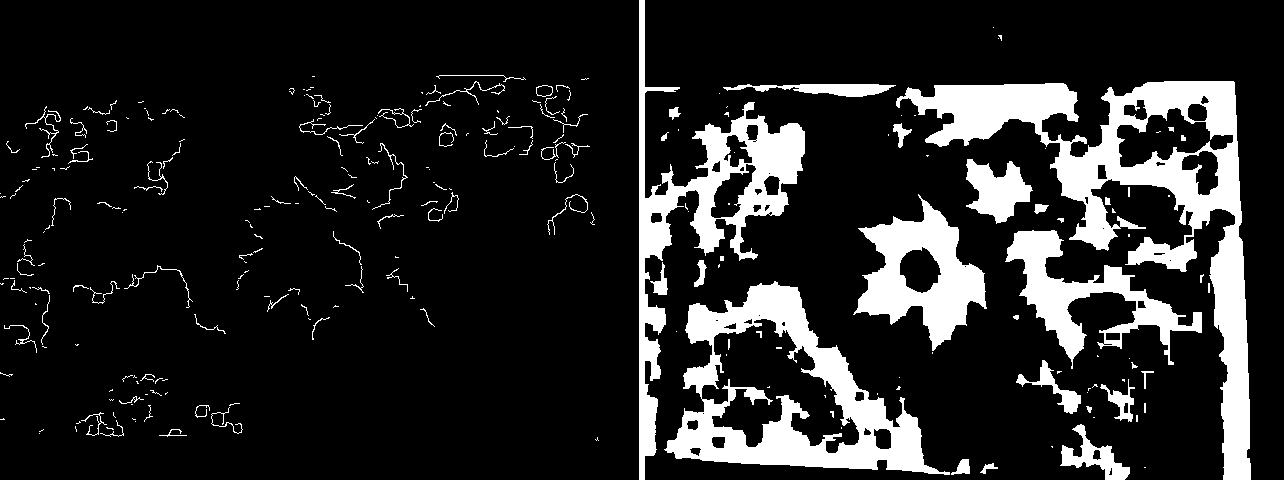
\includegraphics[width=1.0\textwidth]{leaf_identification/images/convert_to_binary.png}
    \caption{Binary image conversion, Canny Edge detection (left) and Adaptive Threshold (right)}%
    \label{preprocessing}
\end{figure}

pg 138

\subsubsection{Edge detection}
pg 153
Canny 

\subsection{Detecting Contours}
A contour is a list of points that represent, in one way or another, a curve in an image \cite{bradski08}. 

pg 251 opencv

\section{Machine Learning Approach}
